\chapter{Application description}\label{chapter:appdescription}

\section{Architecture}
RealityEnhance was developed using Android Studio Flamingo \cite{AndroidStudio}, which is an \ac{IDE} for Android development. The application was developed using Java\cite{Java}, which is a general-purpose programming language.

For the \ac{AR} functionality, the application uses the ARCore software development kit (SDK).
For the \ac{QR} code scanner, the application uses a library called code-scanner \cite{code-scanner}, and for storing the models, the application uses Google Bucket Storage.
As shown in Figure \ref{fig:architecture}, the architecture of the application consists of \ac{APK} that runs on the user's smartphone, which communicates with Google Cloud Storage.

\begin{figure}[ht]
    \centering
    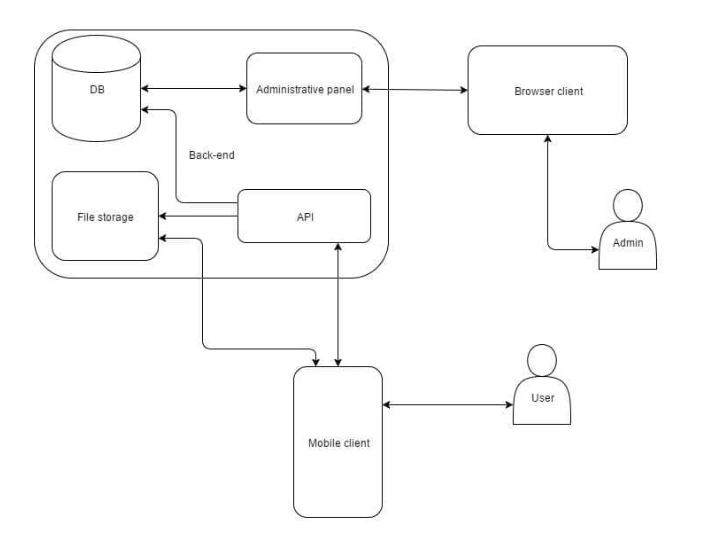
\includegraphics[width=1\textwidth]{img/architecture.png}
    \caption{Architecture}
    \label{fig:architecture}
\end{figure}

\newpage

As shown in Figure \ref{fig:FileStructure}, the file structure of the application consists of the following main folders: java, res and assets. Inside the \textit{java} directory are the main classes of the application (MainActivity, QRActivity, LibraryActivity). Inside the res directory are the resources of the application (icons, layouts, strings). Each layout represents a screen of the application (an Activity). Inside the assets directory are the \ac{3D} models, their images and the tutorial for some of the models. The assets directory is read-only at runtime, so to remove models from the application or add new models, the application will copy the files from assets to the local smartphone storage.

As shown in Figure \ref{fig:Dependencies}, the \textit{build.gradle} file contains the dependencies of the application. Also at the bottom of the figure is the method to generate a \textit{.sfb} file from a \textit{.obj} file. Sceneform supports \ac{3D} assets in the following formats:
\begin{enumerate}
    \item OBJ
    \item glTF (animations not supported)
    \item FBX, with or without animations.
\end{enumerate}
The models can be animated and also they can have textures and custom material\cite{Sceneform}.

\begin{figure}[ht]
    \begin{minipage}{0.5\textwidth}

        \begin{center}
            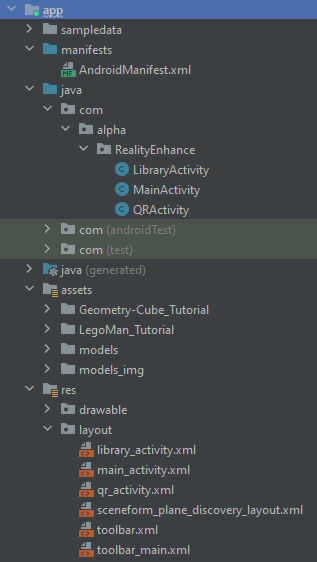
\includegraphics[width=0.65\textwidth]{img/File Structure.png}
            \caption{File Structure}
            \label{fig:FileStructure}
        \end{center}
    \end{minipage}
    \begin{minipage}{0.5\textwidth}
        \begin{center}
            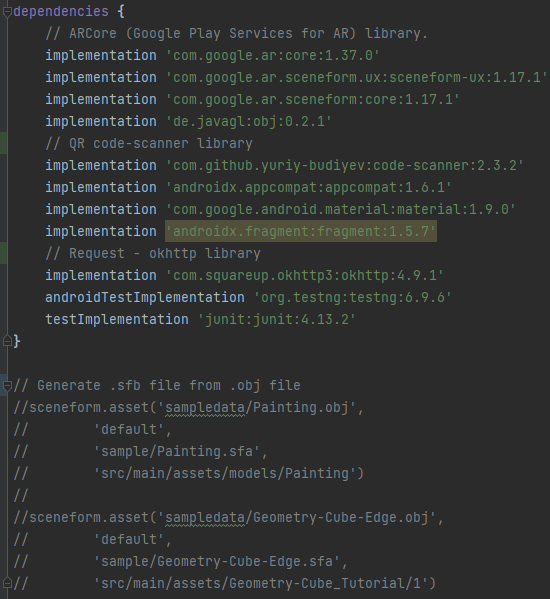
\includegraphics[width=1\textwidth]{img/Dependencies.png}
            \caption{build.gradle file}
            \label{fig:Dependencies}
        \end{center}
    \end{minipage}
\end{figure}




\clearpage

\section{Diagrams}
\subsection*{Class Diagram}
As shown in Figure \ref{fig:ClassDiagram}, the class diagram of the application consists of the following main classes: MainActivity, QRActivity and LibraryActivity.
\par
The MainActivity class is the main class of the application. It is the first class called when the application is started, and it is responsible for the \ac{AR} mode. It contains methods dedicated to interacting with the \ac{3D} models (moving the model, rotating the model, scaling the model).
\par
The QRActivity class is responsible for the \ac{QR} code reader. It has a method called when a \ac{QR} code is scanned and verifies if it is valid. It will check if the model is already imported. If the model is already imported, it will load it from the local storage; it will also request the Google Bucket Storage. Lastly, the LibraryActivity class is responsible for the list of models and the loading of the models.
\begin{figure}[ht]
    \centering
    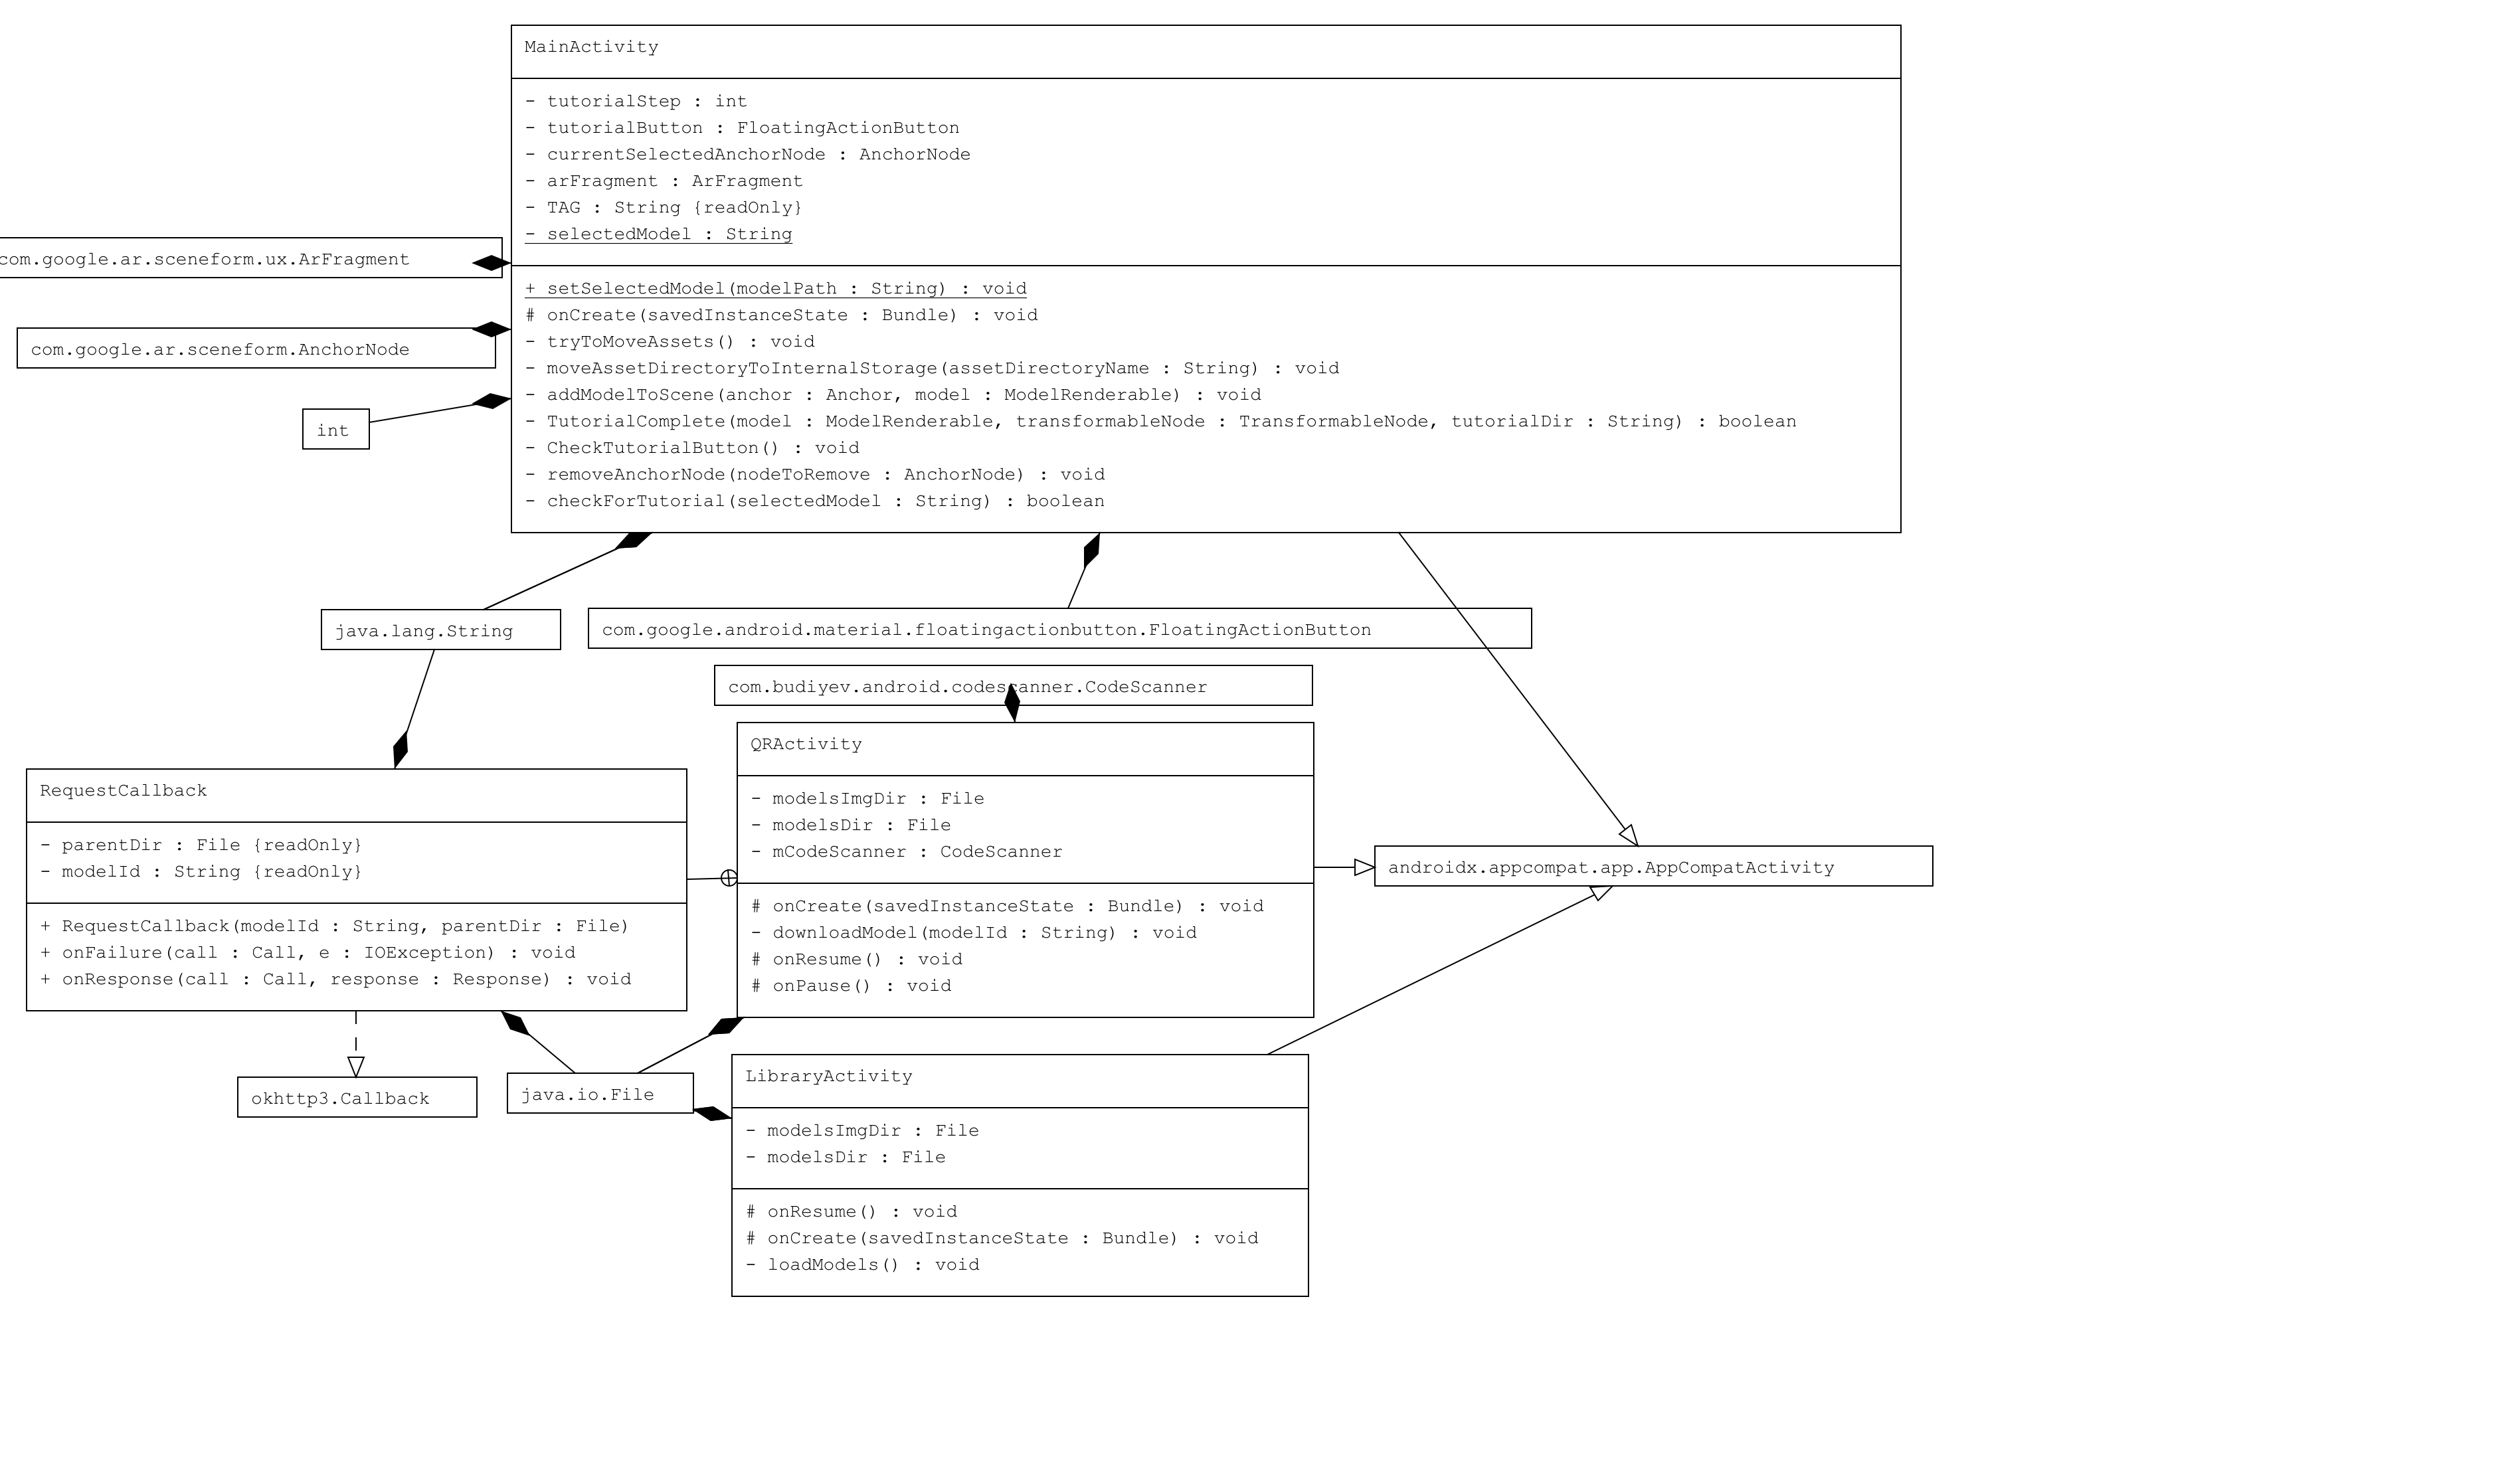
\includegraphics[height=0.9\textwidth]{img/ClassDiagram.png}
    \caption{Class Diagram}
    \label{fig:ClassDiagram}
\end{figure}


\subsection*{Use Case Diagram}
By examining the Use Case Diagram in Figure \ref{fig:UseCaseDiagram}, we gain insights into the functionalities available to users within the application. RealityEnhance allows users to load or import a new model by scanning a \ac{QR} code. Additionally, the application empowers users to engage with the \ac{3D} models in \ac{AR} mode, granting them a dynamic and immersive experience. Furthermore, users can conveniently access a library containing recently used models.

The application's ability to interact with \ac{3D} models is a critical feature. It allows users to explore the models from various perspectives and manipulate their size, orientation, and position through simple gestures. Moreover, users are free to remove any selected model that has already been placed within the \ac{AR} scene, providing them with flexibility and control over their augmented reality experience.
\begin{figure}[ht]
    \centering
    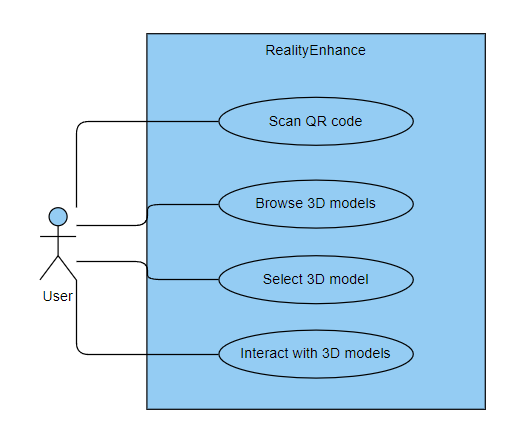
\includegraphics{img/UseCaseDiagram.png}
    \caption{Use Case Diagram}
    \label{fig:UseCaseDiagram}
\end{figure}

\clearpage

\subsection*{Sequence Diagram}
The Sequence Diagram in Figure \ref{fig:SequenceDiagram} shows the interaction between the user and the application. When the user starts the application, a prompt will pop up and request permission to use the camera. After that, the \ac{AR} module will begin to scan the user's surroundings in order to map the environment. For importing a new model, RealityEnhance uses a \ac{QR} code scanner that will check if the code is valid.
\begin{figure}[ht]
    \centering
    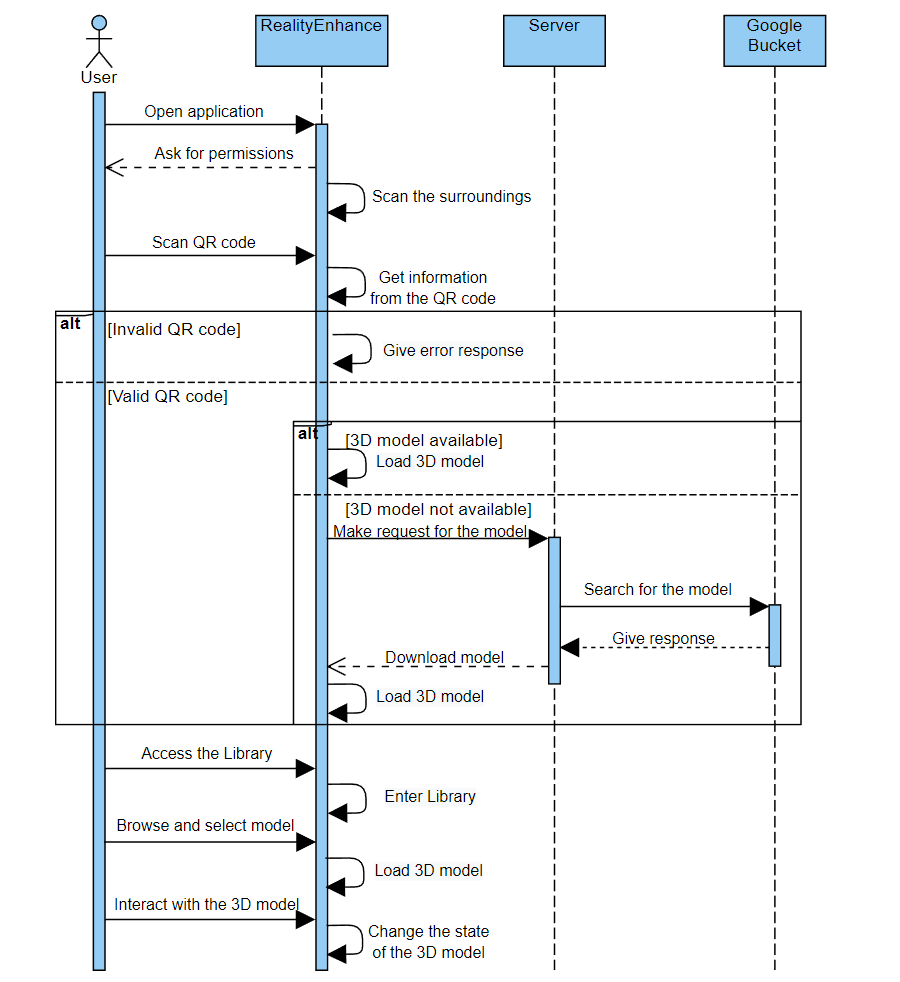
\includegraphics[width=1\textwidth]{img/SequenceDiagram.png}
    \caption{Sequence diagram}
    \label{fig:SequenceDiagram}
\end{figure}
\newpage

If the code fails the validation process, the user is notified and asked to scan another code. If the code is correct, the application will check to see if the model is already in local storage and then load it. If the model is not in the application's local storage, it will send a request to Google Bucket Storage to retrieve all of the model's information (model file, textures, model image, model guide/interactive guide). When the request is completed, a response will be sent back with all of the model's information. The model will then be saved locally and loaded into the \ac{AR} scene.

The user can also browse the Library of already imported models. It also has access to the QR scanner interface and can search for the desired model that is wanted to be loaded in the augmented reality scene. In the \ac{AR} mode, the user is able to place a multitude of models at the same time. These models can be rotated, resized and moved. The interaction between the user and the model bridges the virtual-physical gap and helps build a sense of immersion.

\newpage
\section{Publishing RealityEnhance}
\subsection*{Introduction to App Distribution Platforms}
Developers rely on app distribution platforms to release their applications. The platform they choose greatly impacts their application success. Among the top platforms, Google Play Store and Apple App Store stand out as the go-to choices. These platforms hold immense significance in terms of reaching a vast audience and making an application widely accessible.

\subsection*{Google Play Store}
Google Play Store is the official app store for Android devices\cite{GooglePlay}, offering users a diverse range of applications across various categories. This distribution platform was selected for publishing RealityEnhance because the application was developed for Android devices.

Before publishing an application on Google Play Store, the developers must create a Google Play Console account. The Google Play Console serves as a powerful platform for developers to share and distribute their applications to Android users worldwide. Not only does it provide a convenient way to reach a vast audience, but it also equips developers with a range of tools to expand their user base and generate revenue.

Accessing the Google Play Console is a breeze since it is a web-based platform, as shown in Figure \ref*{fig:GooglePlayConsole}. However, before publishing anything on the Google Play Store, it is crucial to ensure that the application is properly prepared for release. Taking the necessary steps to prepare the application will help guarantee a smooth and successful launch on the platform. The developer must have a specific file structure and then create a signed bundle file. After the bundle file is created and validated by Google Play Console, the application can be published.

\begin{figure}[ht]
    \centering
    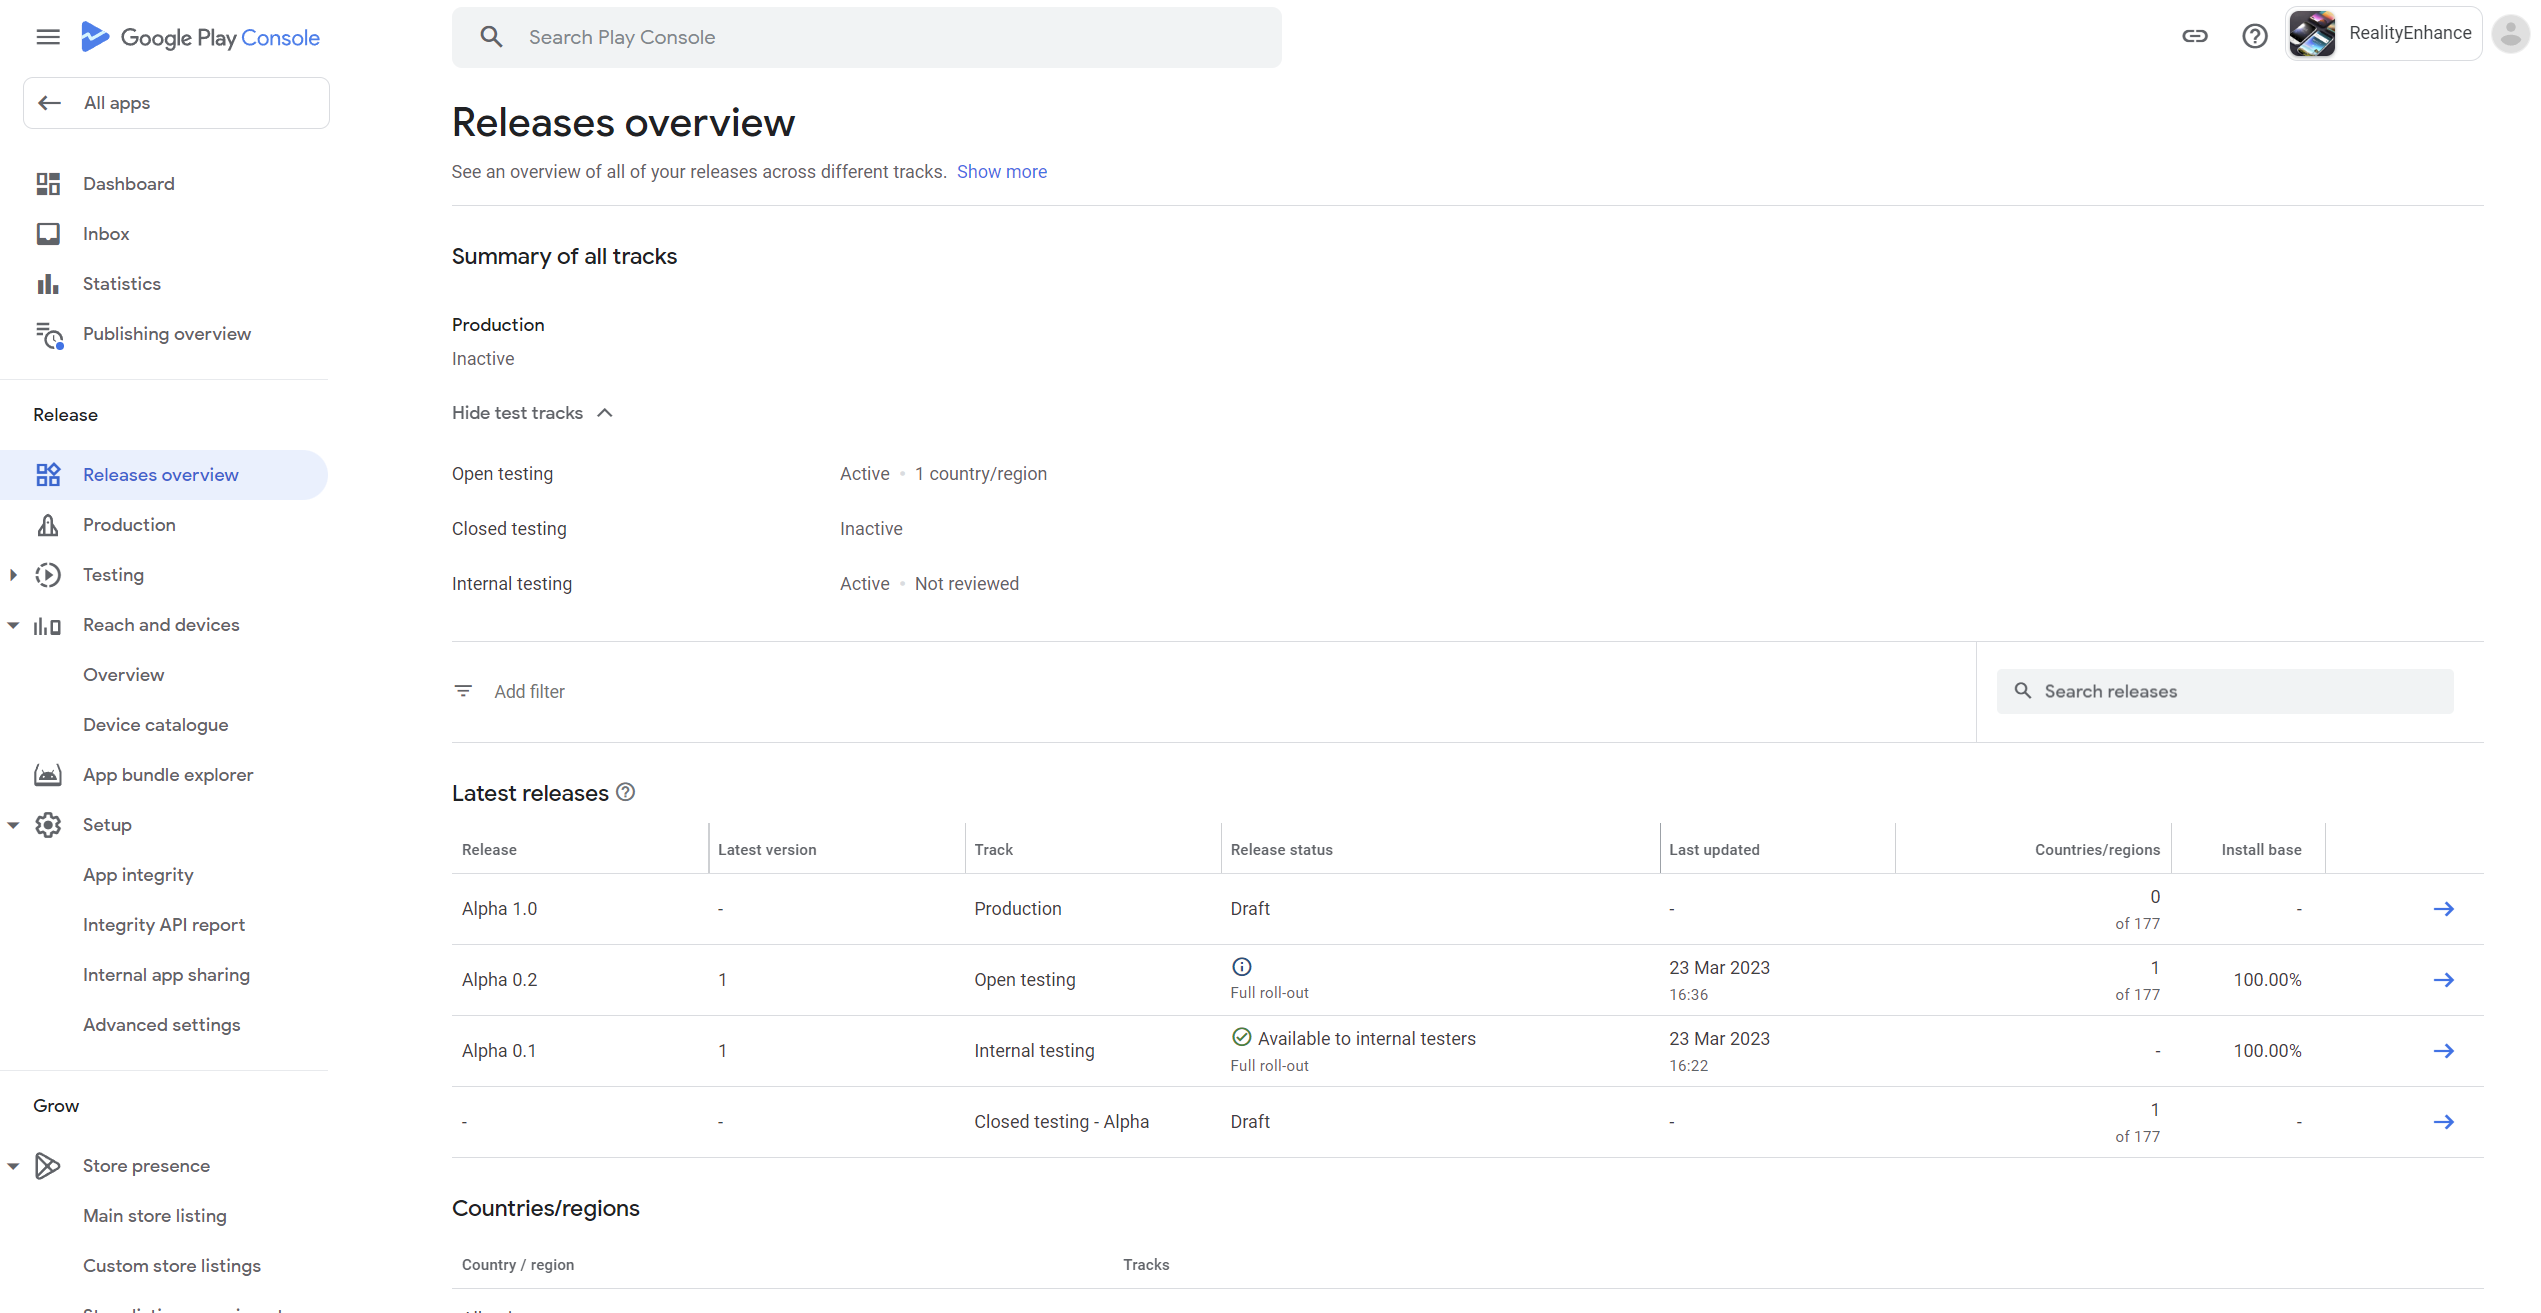
\includegraphics[width=.9\textwidth]{img/GooglePlayConsole.png}
    \caption{Google Play Console}
    \label{fig:GooglePlayConsole}
\end{figure}